\section{Visualizer Packages}
One of the most essential goals for BNumMet was to provide a graphical user interface that will allow students to view one or more parts of an underlying algorithm, with the goal of encouraging students to learn such algorithms.

In our quest to create this graphical user interface, we must keep in mind that, while the Python programming language excels in many areas such as data analysis, artificial intelligence, basic scripting, and so on, Python is not currently suitable - in general - for creating the graphical user interfaces that we are accustomed to seeing in our daily lives. It definitely includes modules for such jobs (PyQt, SimpleGUI,...), but Python was not designed with such in mind. To that purpose, as stated in J.C. Bucheli's work, we will be utilizing Jupyter Notebooks, an external Python Library that offers a more natural view of the code as if it were some class notes. We will leverage the widgets provided by both iPyWidgets and BQPlot in this Jupyter notebook to enhance the capability of the notebook, in our instance, with  interactivity.  The rationale for adopting the same approach as J.C. Bucheli is that Jupyter is still extensively used in both the scientific and industrial communities for displaying code in an easy-to-read style and for correctly teaching coding skills to students.

Overall, the following packages will be an expansion to the approaches described previously in a format that will improve understanding without requiring an installation outside of what is generally installed and in a format that students will be accustomed to in their professional and academic life.

It is worth mentioning that most of the implementations had the core principles of what Mathworks sought to represent, but we have tried to focus on resolving some of the flaws that may prevent students from seeing the functionality effectively. Furthermore, all of the techniques supplied present default situations in case students just wish to check out the visualizer without thinking about examples.

\subsection{LU Visualizer}
As both Mathworks and J.C. Bucheli's work had implemented, we will strive to improve on the current visualizers made; however, before we start, we must discuss what is the underlying idea and some of the shortcomings that each had before to adopting this new visualizer.

The LU Visualizer's purpose will be to implement a graphical user interface that presents the main steps of the LU decomposition, which are pivot selection and reduction; additionally, at the end of the decomposition, the matrices that represent the permutation and the lower and upper triangular parts must be shown. 

On the one hand, Mathworks performed an excellent job of creating the visualizer, allowing users to pick the pivot for each row and then do computations, as well as displaying an automated LU decomposition with three major methods: diagonal, partial, and complete pivoting. It's worth noting that this visualizer uses the standard LU Decomposition we have also implemented as a method without the rank revealing mechanism. Furthermore, it does not specify which pivots are accessible at each step \imgref{fig:Mathworks Example 1 - No help in pivots to choose}, not to mention that this work permitted the LU method to use zero as a pivot element, resulting in $NaN$ and $Inf$ values, which are not appropriate for a student to understand \imgref{fig:Mathworks Example 1 - No help in pivots to choose}. It also does not display the permutation matrix and does not adequately identify which matrix is the L or U matrix, which is inconvenient for students.

 
\begin{figure}[H]
    \centering
    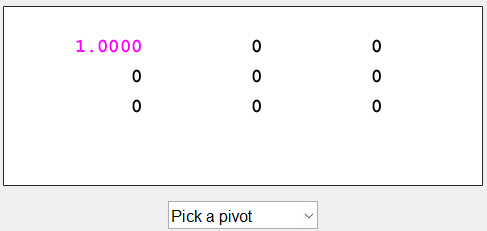
\includegraphics[scale=0.7]{Include/Images/Thesis/Development/Visualizers/LU VISUALIZER/Mathworks.LU.Ex1.png}
    \caption{Mathwork's \cite{doi:10.1137/1.9780898717952} Example 1 - No help in pivots to choose}
    \label{fig:Mathworks Example 1 - No help in pivots to choose}
\end{figure}

\begin{figure}[H]
    \centering
    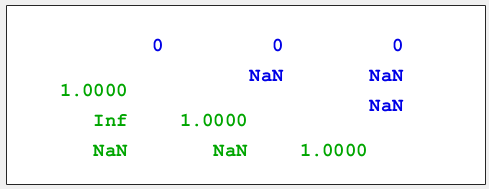
\includegraphics[scale=0.7]{Include/Images/Thesis/Development/Visualizers/LU VISUALIZER/Mathworks.LU.Ex1.1.png}
    \caption{Mathwork's \cite{doi:10.1137/1.9780898717952} Example 1 - Nan and inf values}
    \label{fig:Mathworks Example 1 - Nan and inf values}
\end{figure}


On the other side, while several of the issues raised in the Mathworks case were addressed in J.C. Bucheli's work, such as a visual assistance on which pivots may be clicked on, we were unable to use this visualizer, which appears to be malfunctioning with no error signals given. On that point, a deeper examination of J.C. Bucheli's code revealed the usage of threading techniques, which may be improper to maintain as well as inadequate for this sort of algorithm, because the LU algorithm does not require an external process to perform the modifications at each step. Furthermore, a timer was provided for the user to pick, which is contrary to acceptable standards in the development of a user G.U.I.

\begin{figure}[H]
    \centering
    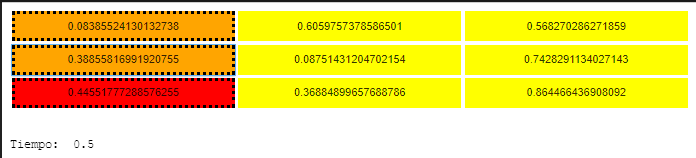
\includegraphics[width=\textwidth]{Include/Images/Thesis/Development/Visualizers/LU VISUALIZER/Camilo.LU.Ex1.png}
    \caption{J.C. Bucheli's \cite{bucheli2020} LU Visualizer Example 1}
    \label{fig:J.C. Bucheli's LU Visualizer Example 1}
\end{figure}


Once we know what are the main critiques of previously done work we can proceed by commenting on the proposed solution. 
\begin{figure}[H]
    \centering
    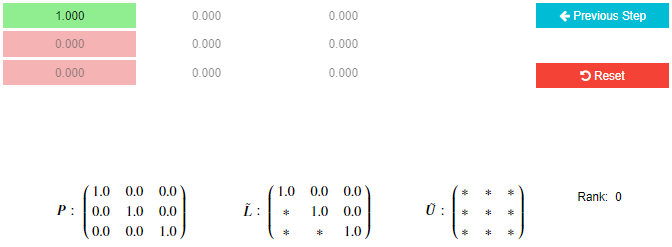
\includegraphics[width=\textwidth]{Include/Images/Thesis/Development/Visualizers/LU VISUALIZER/BNumMet.LU.Ex1.png}
    \caption{BNumMet Example 1}
    \label{fig:BNumMet Example}
\end{figure}

As we can see, unlike Mathworks, the end-user knows which elements can be selected to pivot, and it prevents the user from dividing by zero, as well as the current output of the P,L,U matrices at each step (note the asterisk to indicate that we do not know the value at that step and it remains to be calculated). We additionally highlight two buttons, "Previous Step" and "Reset," because a user may miss click a button and not reach their intended aim, and we want pupils to feel comfortable when using our interactive visualizer.
Furthermore, we indicate the rank we can guarantee the matrix has at each iteration by implementing the rank revealing mechanism, and the final result will be indicated by a system message \imgref{fig:BNumMet Example End Result}. Note that if the LU finds a column of possible pivots to be zero during the iterations, it will send a message as a system message explaining to the user that the algorithm has jumped the column until it finds a suitable one to pivot.

\begin{figure}[H]
    \centering
    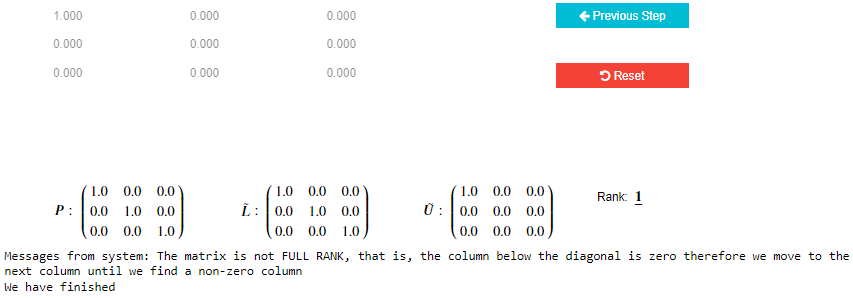
\includegraphics[width=\textwidth]{Include/Images/Thesis/Development/Visualizers/LU VISUALIZER/BNumMet.LU.Ex1.1.png}
    \caption{BNumMet LU Visualizer Example End Result}
    \label{fig:BNumMet Example End Result}
\end{figure}

Overall, the proposed solution corrects the previously done work while also improving it by providing the properties of the LU algorithm at a glance (Rank revealing, matrices at each iteration) and by improving the majority of the visual aspect of the overall implementation.

\subsubsection{Examples}
	\paragraph{Example 1: No arguments}{
\begin{lstlisting}[language=Python]
from BNumMet.Visualizers.LUVisualizer import LUVisualizer
luVisualizer = LUVisualizer()
display(luVisualizer.run())
\end{lstlisting}

\begin{enumerate}
  \item Initial State:\\  
    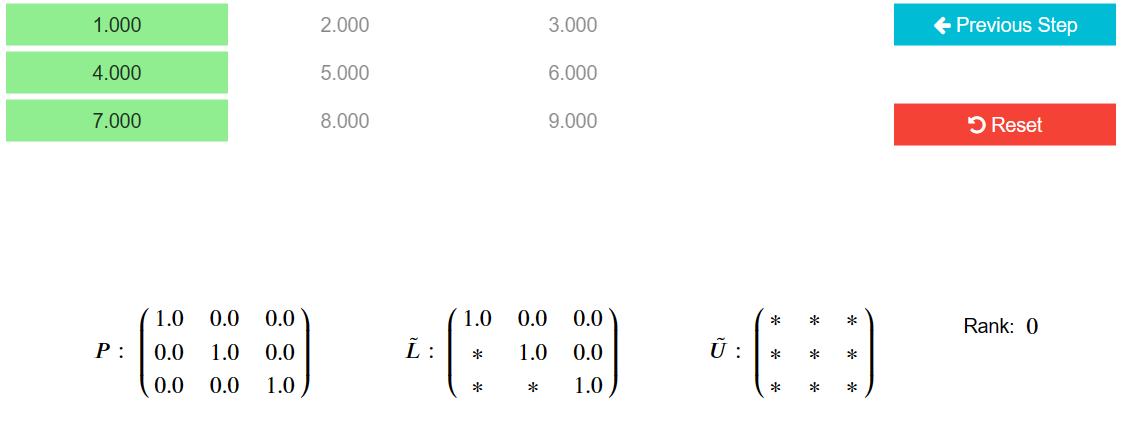
\includegraphics[scale=0.45]{Include/Images/Thesis/Documentation/Visualizers/LUVisualizer/Example 1/Example 1 - 00 - Initial State.png}
  \item Click on first column, second row:\\
    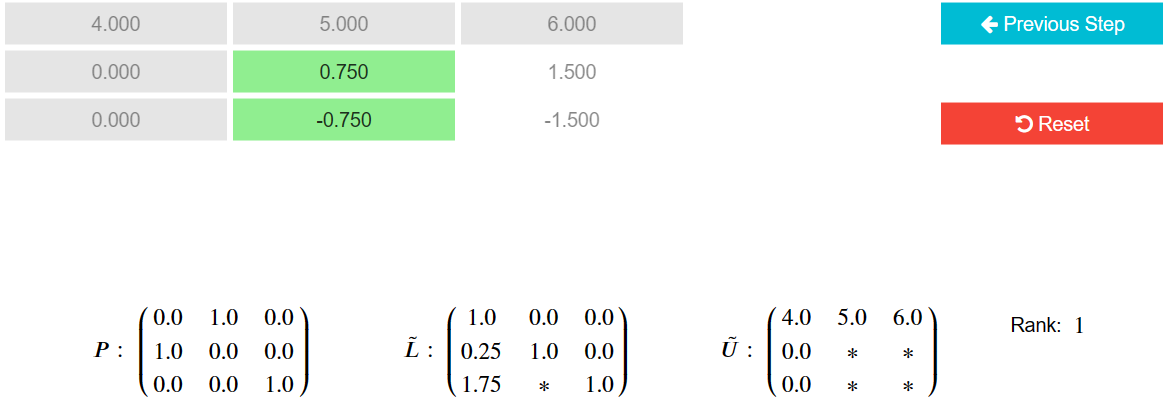
\includegraphics[scale=0.45]{Include/Images/Thesis/Documentation/Visualizers/LUVisualizer/Example 1/Example 1 - 01 - Click on 2 row.png}
  \item Click on second column, third row:\\
    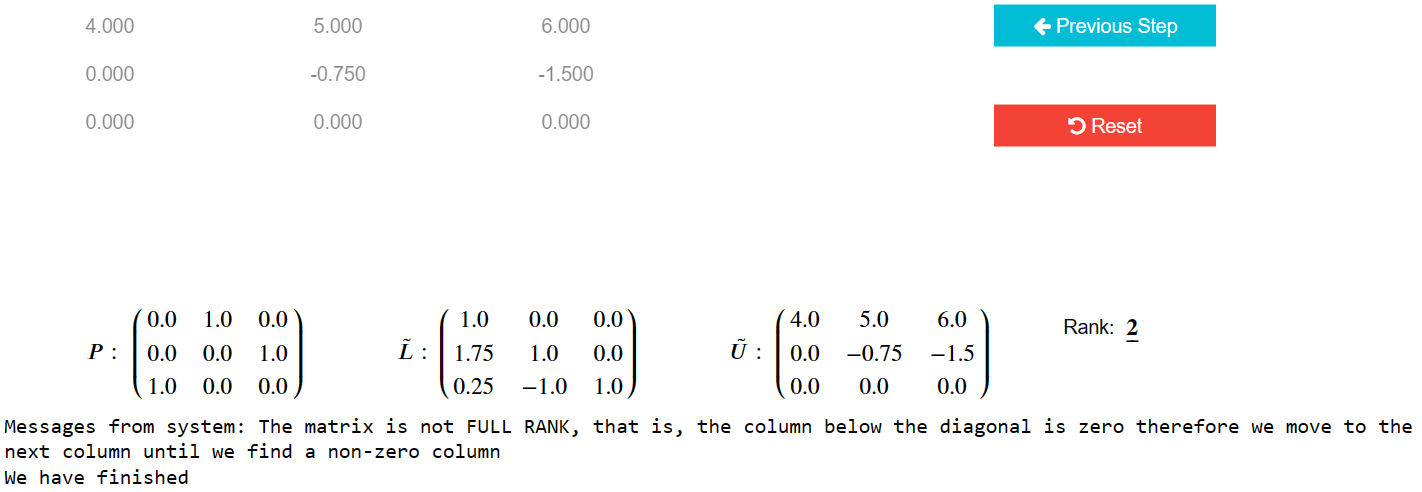
\includegraphics[scale=0.4]{Include/Images/Thesis/Documentation/Visualizers/LUVisualizer/Example 1/Example 1 - 02 - Click on 3 row.png}
  \item Click Previous Step:\\
    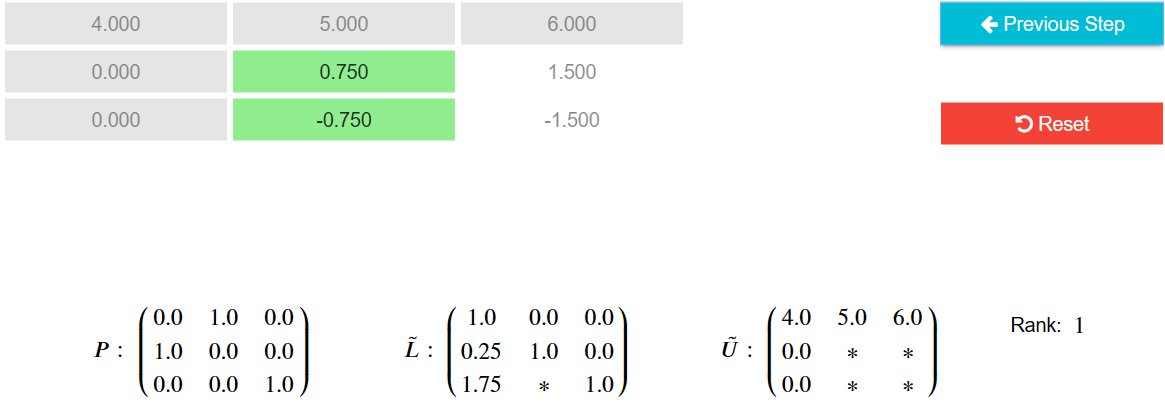
\includegraphics[scale=0.45]{Include/Images/Thesis/Documentation/Visualizers/LUVisualizer/Example 1/Example 1 - 03 - Click Previous Step.png}
  \item Click on second column, second row:\\
    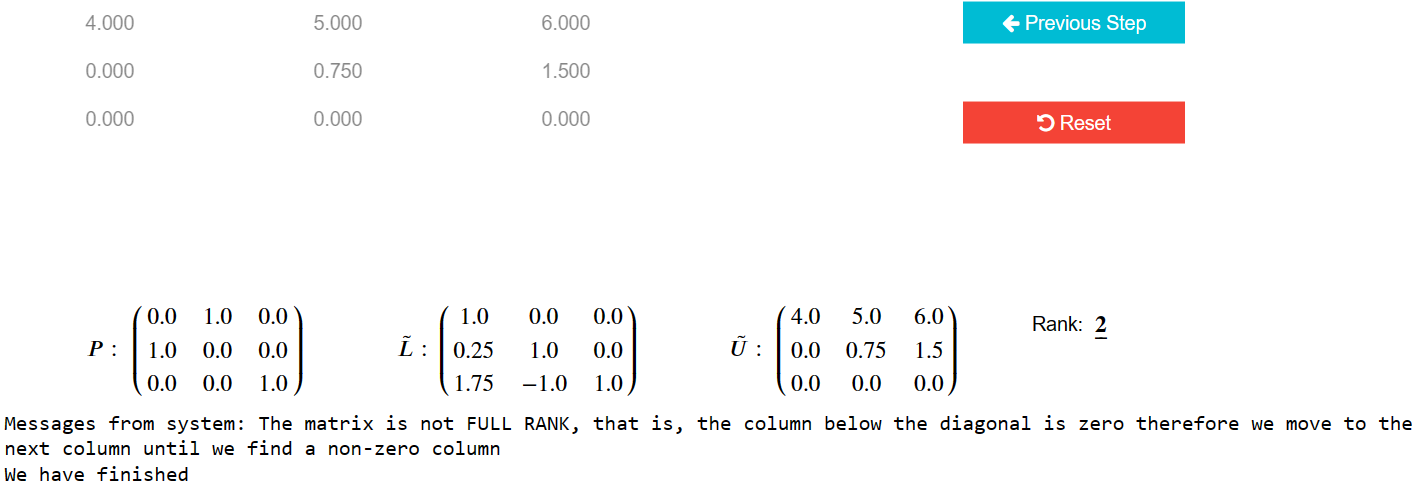
\includegraphics[scale=0.4]{Include/Images/Thesis/Documentation/Visualizers/LUVisualizer/Example 1/Example 1 - 04. - Click on 2 row.png}
  \item Click on Reset\\
      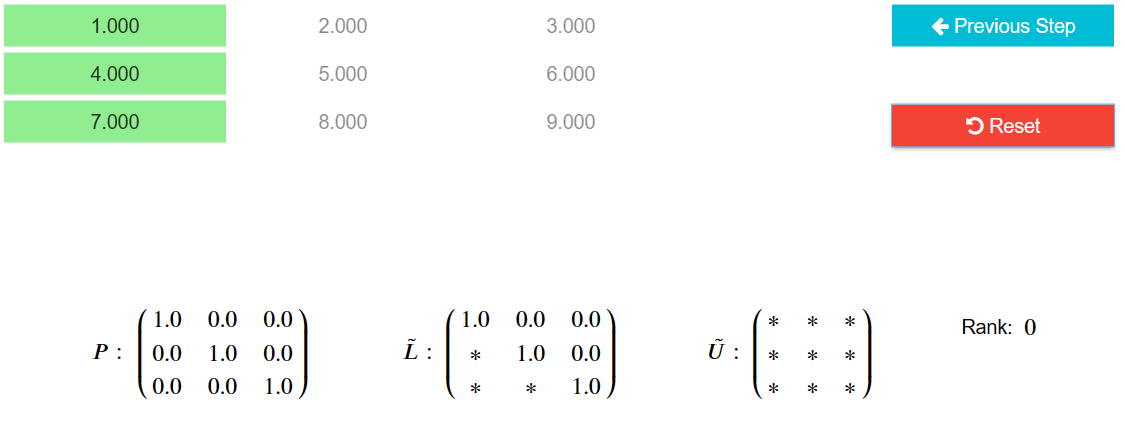
\includegraphics[scale=0.45]{Include/Images/Thesis/Documentation/Visualizers/LUVisualizer/Example 1/Example 1 - 05 - Click on Reset.png}
\end{enumerate}
}
\paragraph{Example 2: Arguments and Rank Revealing}{
\begin{lstlisting}[language=Python]
from BNumMet.Visualizers.LUVisualizer import LUVisualizer
A = np.array([[1,2,3,7], [1,2,3,7], [1,2,3,7],[1,2,4,7]], dtype=float)
luVisualizer = LUVisualizer(A)
display(luVisualizer.run())
\end{lstlisting}

\begin{enumerate}
\item Initial State: \\
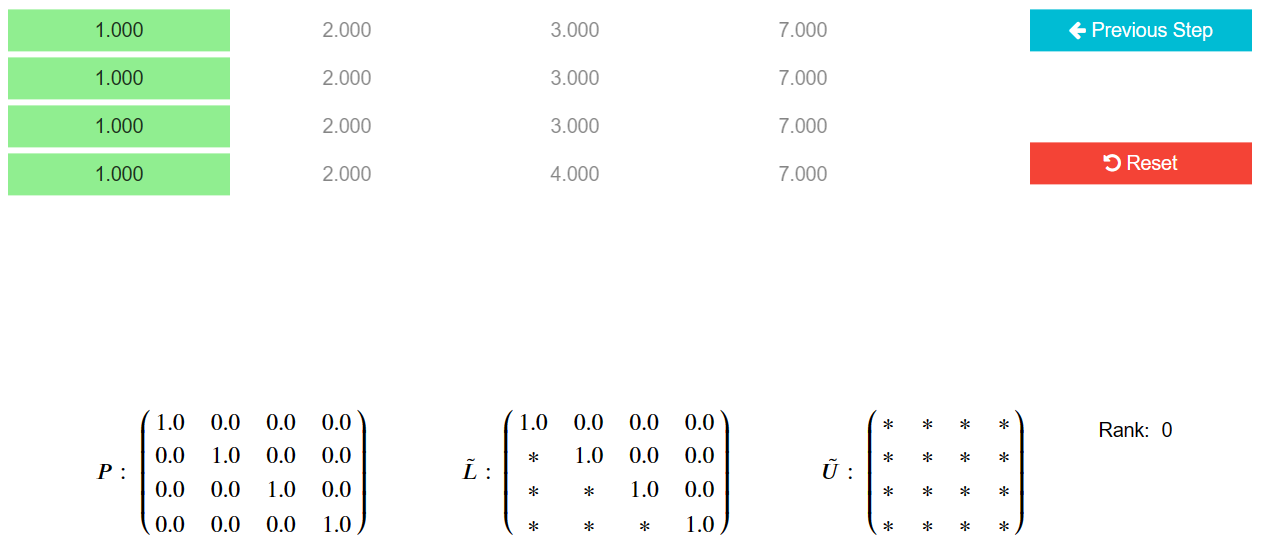
\includegraphics[scale=0.45]{Include/Images/Thesis/Documentation/Visualizers/LUVisualizer/Example 2/Example 2 - 00 - Initial State.png}

\item Click on the first column, second row: \\
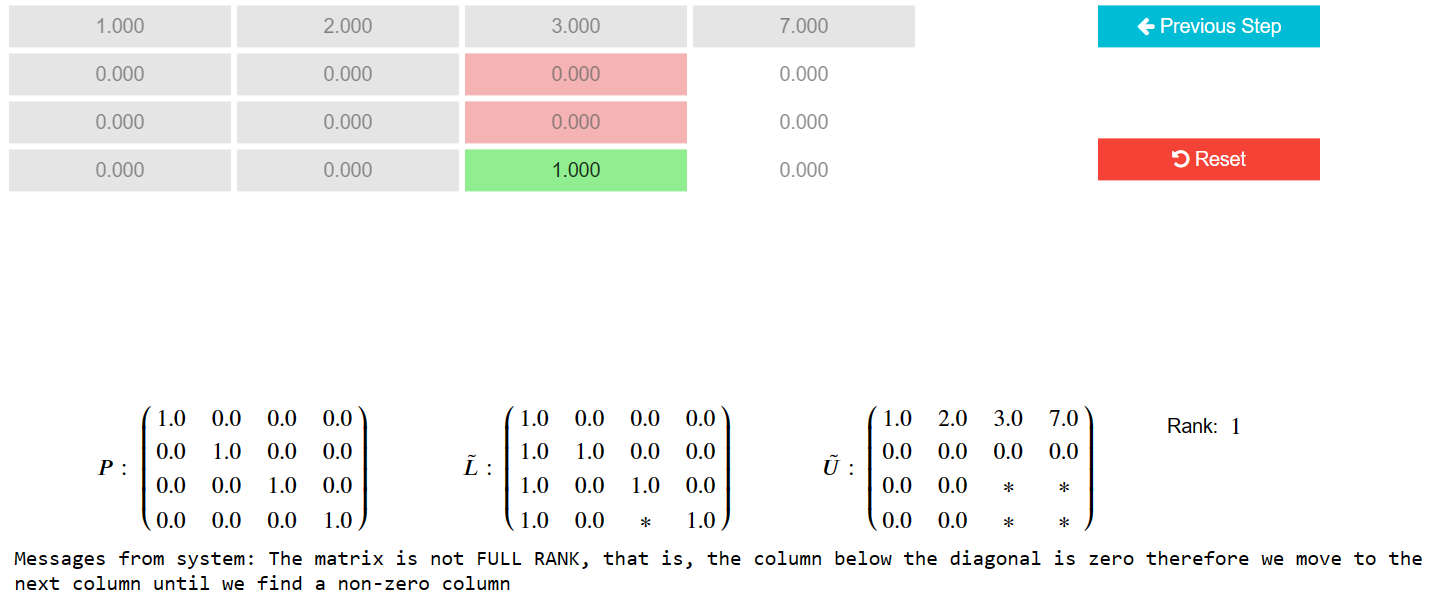
\includegraphics[scale=0.4]{Include/Images/Thesis/Documentation/Visualizers/LUVisualizer/Example 2/Example 2 - 01 - Click first column, second row.png}

\item Click on the third column, fourth row: \\
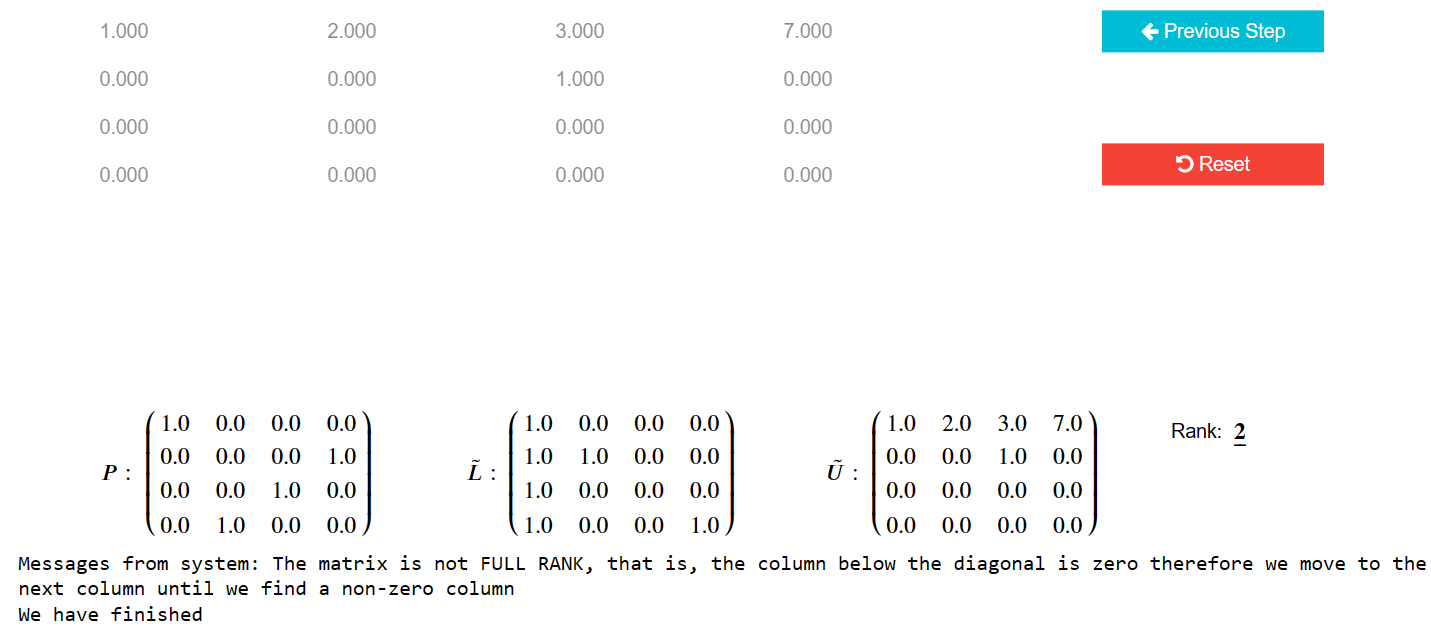
\includegraphics[scale=0.4]{Include/Images/Thesis/Documentation/Visualizers/LUVisualizer/Example 2/Example 2 - 02 - Click thirdcolumn, fourth row.png}
\end{enumerate}
}


\subsection{Interpolation Visualizer}
As with the LU Visualizer, we will begin by discussing previous works and potential areas for improvement.

The interpolation visualizer's goal is to demonstrate the viewer how different interpolation methods compare to one another, as well as how moving the dataset or adding points might affect the initial interpolation given.

To begin, we will highlight Mathwork's implementation, which allows the user to select different interpolation methods while also allowing the user to edit the points and observe the changes. Despite the excellent implementation, it lacks the ability to add more points at runtime and does not allow viewing the entire interpolation when the function exceeds the limits set by the initial plot \imgref{fig:Mathwork's Interpolation Example - Drawbacks},  it also has some bad contrast between the text and the background (on the text "poly"), and this does not obey the Human-Computer Interaction good practices. We must also emphasize the reset button, which may be useful to students if they accidentally change a point. 

\begin{figure}[H]
    \centering
    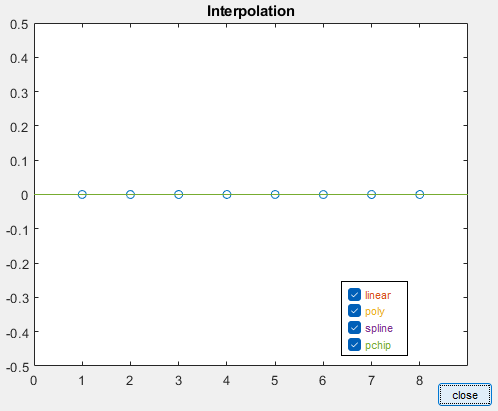
\includegraphics[width=0.6\textwidth]{Include/Images/Thesis/Development/Visualizers/INTERPOLATION VISUALIZER/Mathworks.Interpolation.Ex1.png}
    \caption{Mathwork's \cite{doi:10.1137/1.9780898717952} Interpolation Example}
    \label{fig:Mathworks Interpolation Example}
\end{figure}
\begin{figure}[H]
    \centering
    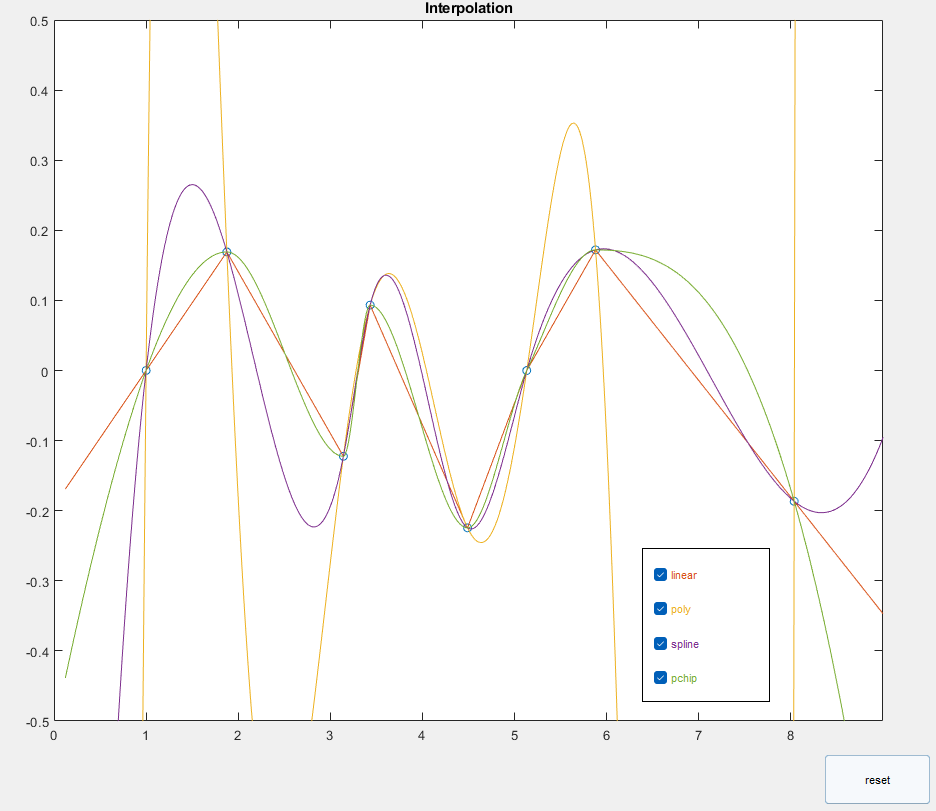
\includegraphics[width=\textwidth]{Include/Images/Thesis/Development/Visualizers/INTERPOLATION VISUALIZER/Mathworks.Interpolation.Ex1.1.png}
    \caption{Mathwork's \cite{doi:10.1137/1.9780898717952} Interpolation Example - Drawbacks}
    \label{fig:Mathwork's Interpolation Example - Drawbacks}
\end{figure}


Secondly, concentrating on J.C. Bucheli's effort, we must emphasize that the implementation was not completed, thus any comments will be based on what seems to be implemented. To begin, we should observe that the visualization does not support various interpolation methods; nevertheless, unlike Mathworks, this solution allows for plot movement but not single point movement or addition of points, as we can observe \imgref{fig:Camilo's Interpolation Visualizer Example - Drawbacks} moving the points will not update the plot.

\begin{figure}[H]
    \centering
    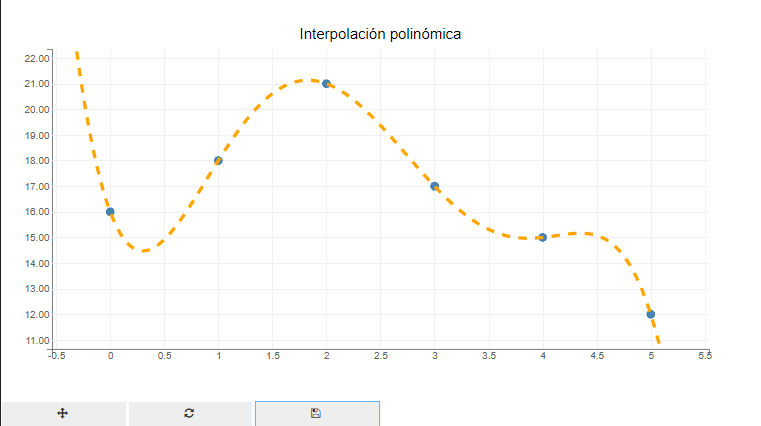
\includegraphics[width=\textwidth]{Include/Images/Thesis/Development/Visualizers/INTERPOLATION VISUALIZER/Camilo.Interpolation.Ex1.png}
    \caption{J.C. Bucheli's \cite{bucheli2020} Interpolation Visualizer Example}
    \label{fig:J.C. Bucheli's Interpolation Visualizer Example}
\end{figure}

\begin{figure}[H]
    \centering
    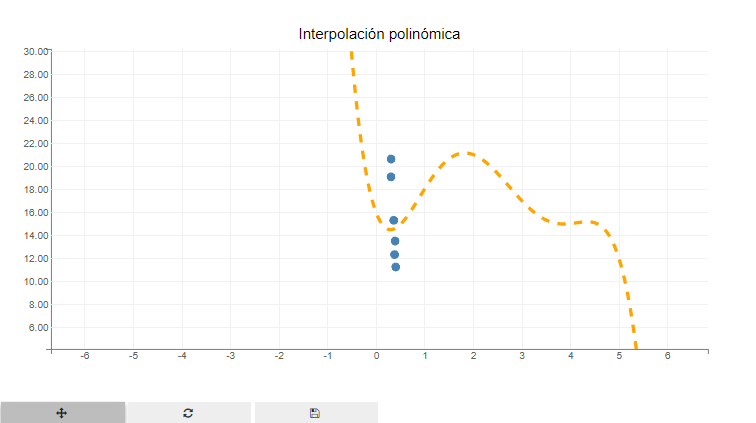
\includegraphics[width=\textwidth]{Include/Images/Thesis/Development/Visualizers/INTERPOLATION VISUALIZER/Camilo.Interpolation.Ex1.1.png}
    \caption{J.C. Bucheli's \cite{bucheli2020} Interpolation Visualizer Example - Drawbacks}
    \label{fig:J.C. Bucheli's Interpolation Visualizer Example - Drawbacks}
\end{figure}


After understanding the important aspects and critiques of the preceding discussion, we create our own implementation, keeping in mind that numerous interpolating methods should be accessible to pick from, it should be able to move and add points, and it should include a button to undo all changes done.
\begin{figure}[H]
    \centering
    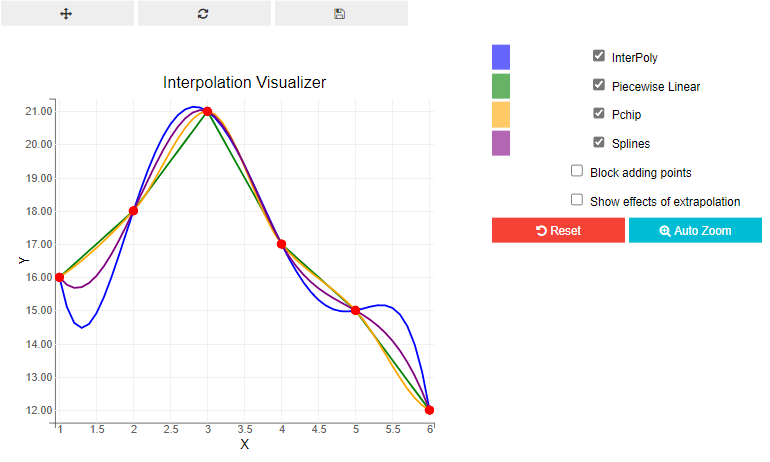
\includegraphics[width=\textwidth]{Include/Images/Thesis/Development/Visualizers/INTERPOLATION VISUALIZER/BNumMet.Interpolation.Ex1.png}
    \caption{BNumMet Interpolation Visualizer Example}
    \label{fig:BNumMet Interpolation Visualizer Example}
\end{figure}
As we can see, it has a similar appearance to Mathwork's implementation, but it adds an auto-zoom button in the case of out-of-bounds graphs \imgref{fig:BNumMet Interpolation Visualizer Example - Adding points and auto zooming}, as well as two check boxes, one that prevents the user from adding more points if the user decides to move the graph, and "show extrapolation effects", which shows the user what effects the extrapolation has on attempting to predict the "past" or "future"  \imgref{fig:BNumMet Interpolation Visualizer Example - Extrapolation}. 
\begin{figure}[H]
    \centering
    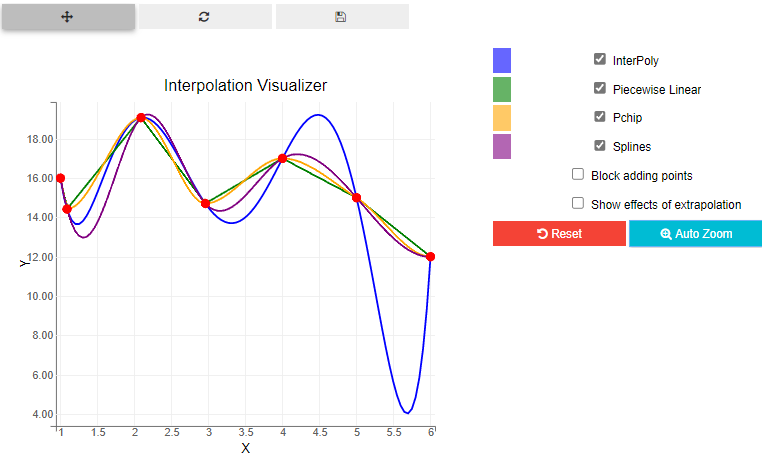
\includegraphics[width=\textwidth]{Include/Images/Thesis/Development/Visualizers/INTERPOLATION VISUALIZER/BNumMet.Interpolation.Ex1.1.png}
    \caption{BNumMet Interpolation Visualizer Example - Adding points and auto zooming}
    \label{fig:BNumMet Interpolation Visualizer Example - Adding points and auto zooming}
\end{figure}
\begin{figure}[H]
    \centering
    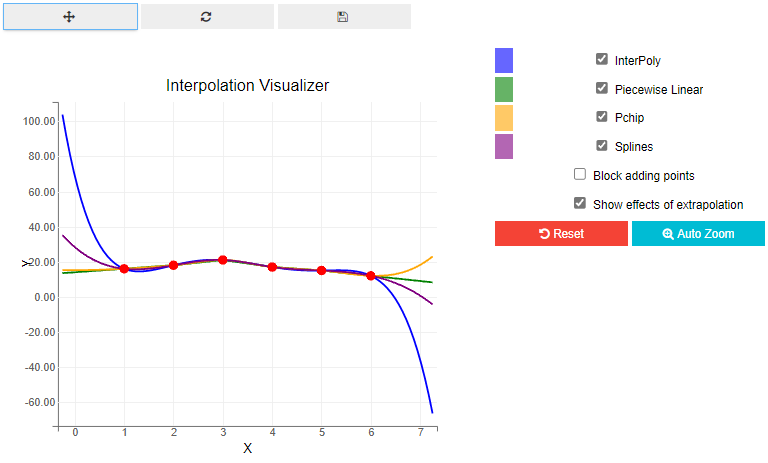
\includegraphics[width=\textwidth]{Include/Images/Thesis/Development/Visualizers/INTERPOLATION VISUALIZER/BNumMet.Interpolation.Ex1.2.png}
    \caption{BNumMet Interpolation Visualizer Example - Extrapolation}
    \label{fig:BNumMet Interpolation Visualizer Example - Extrapolation}
\end{figure}

Overall, we reckon that the method supplied corrects some of the minor flaws raised by Mathwork's approach while also providing some concepts that may assist academics in explaining why interpolation should not be utilized for extrapolation. 
\subsubsection{Examples}
	\paragraph{Example 1}
\begin{lstlisting}[language=Python]
from BNumMet.Visualizers.InterpolationVisualizer import InterpolVisualizer
interpolVisualizer = InterpolVisualizer()
display(interpolVisualizer.run())
\end{lstlisting}
\begin{enumerate}
\item Initial State: \\
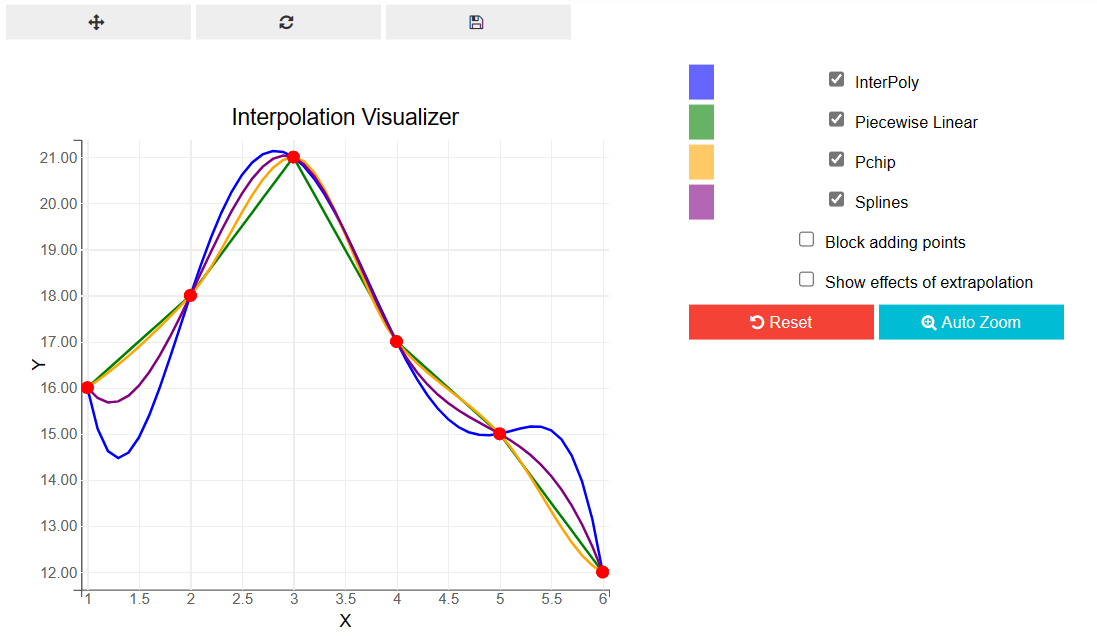
\includegraphics[scale=0.5]{Include/Images/Thesis/Documentation/Visualizers/Interpolation/Example 1/Example 1 - 00 - Initial State.png}

\item Checked Box Extrapolation and AutoZoom: \\
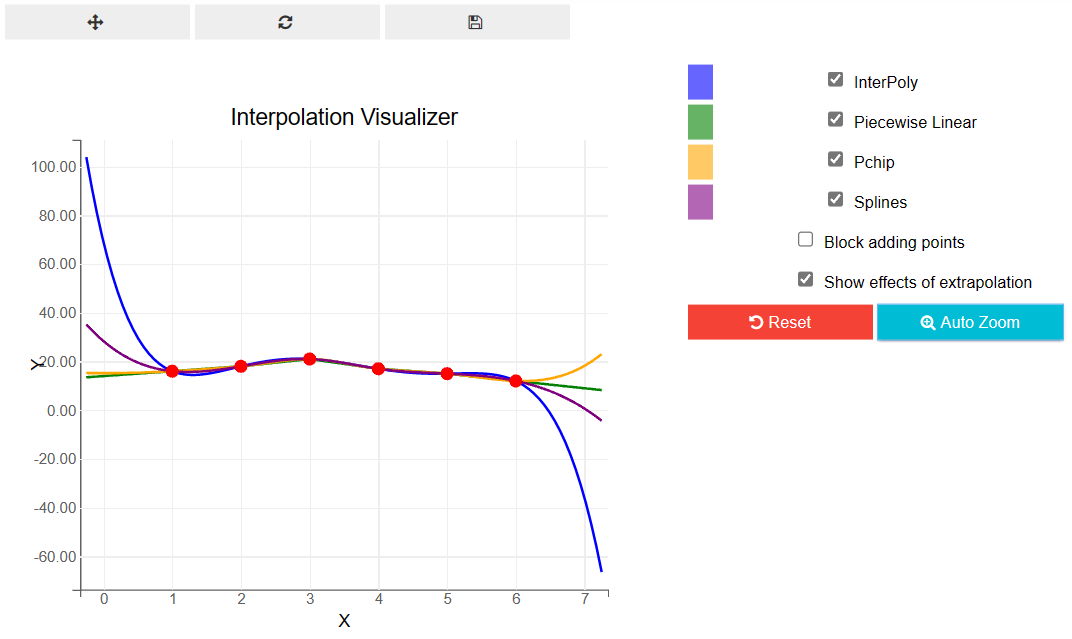
\includegraphics[scale=0.5]{Include/Images/Thesis/Documentation/Visualizers/Interpolation/Example 1/Example 1 - 01 - Checked Box Extrapolation and AutoZoom.png}

\item Reset Button: \\
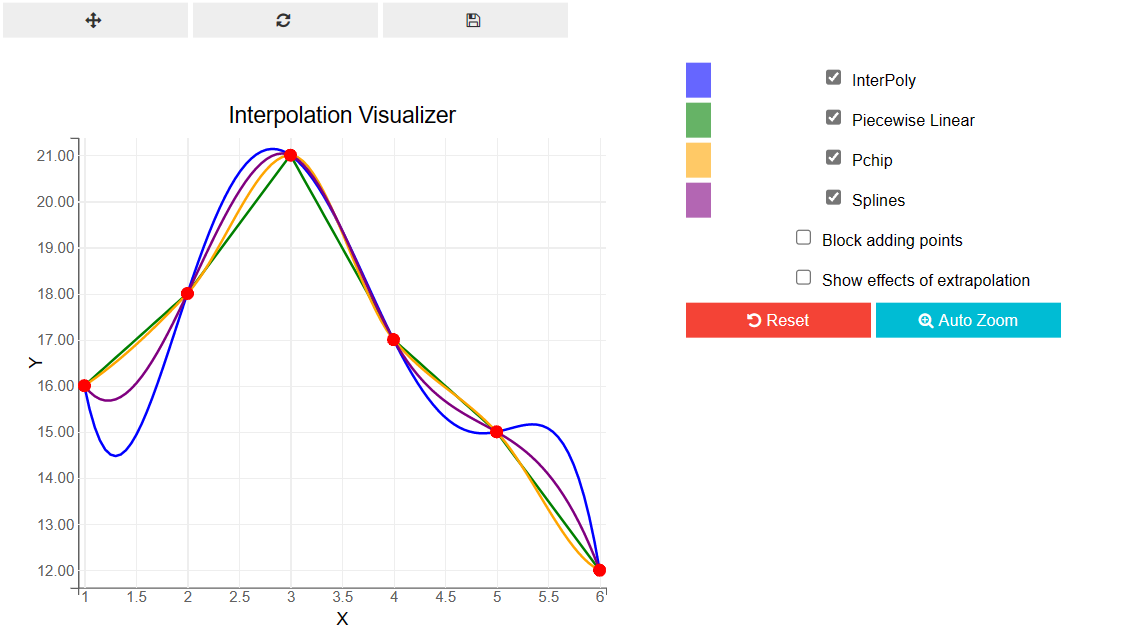
\includegraphics[scale=0.5]{Include/Images/Thesis/Documentation/Visualizers/Interpolation/Example 1/Example 1 - 02 - Reset Button.png}

\item Added Point: \\
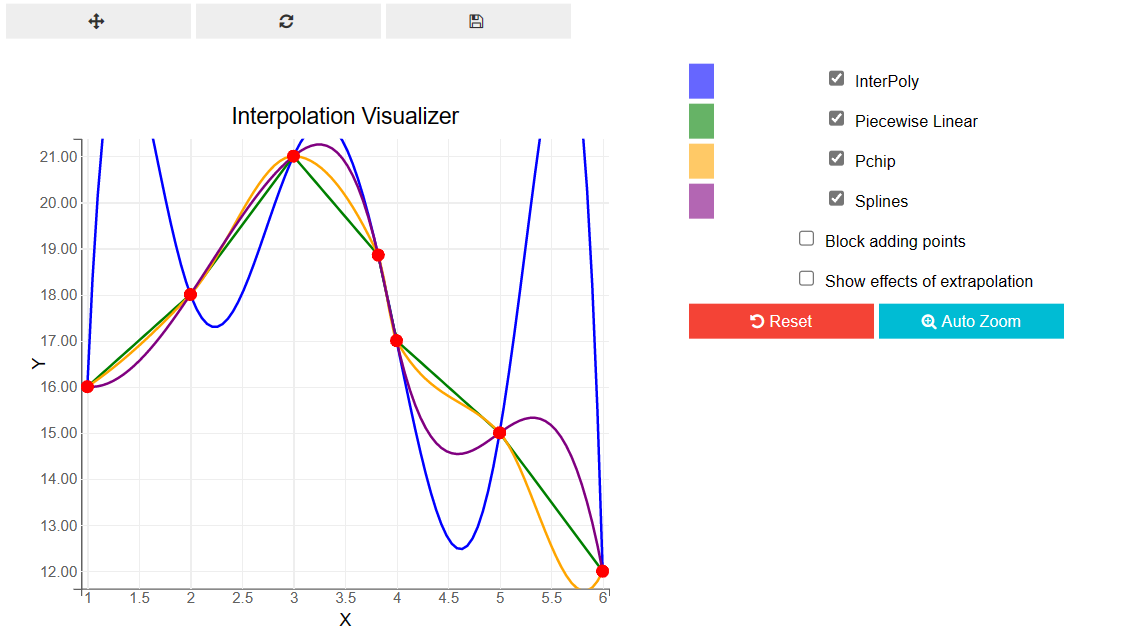
\includegraphics[scale=0.5]{Include/Images/Thesis/Documentation/Visualizers/Interpolation/Example 1/Example 1 - 03 - Added Point.png}

\item AutoZoom: \\
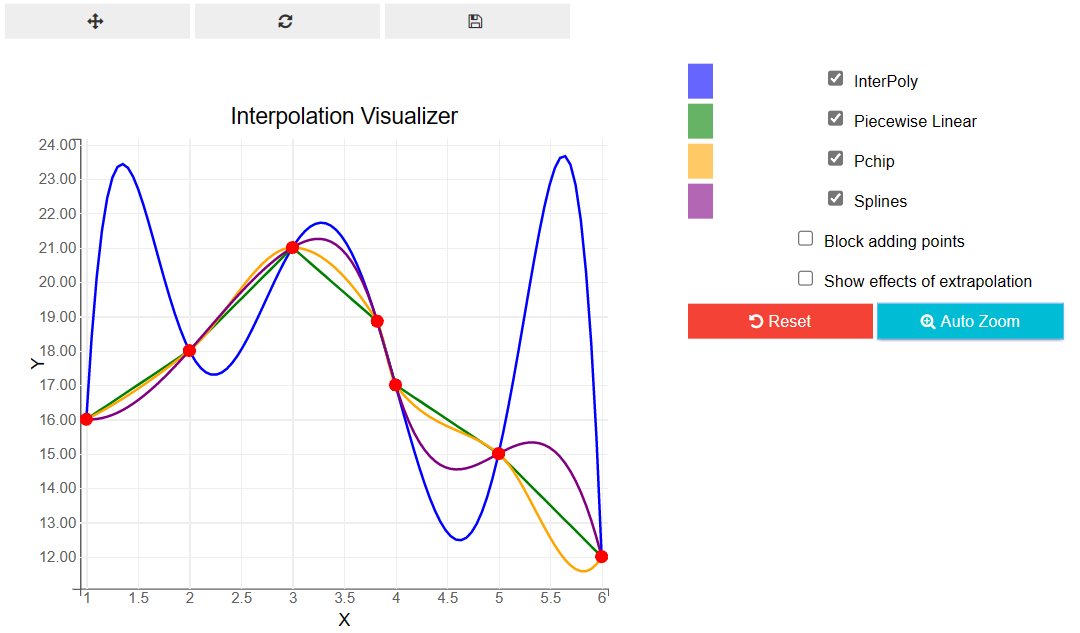
\includegraphics[scale=0.5]{Include/Images/Thesis/Documentation/Visualizers/Interpolation/Example 1/Example 1 - 04 -AutoZoom.png}
\end{enumerate}

\subsection{Non Linear Equation Solver Visualizer}
Continuing with our visualizers, we have also implemented an interactive visualization for the Non Linear Equation Solver Package. As before, we will first discuss the considerations taken by Mathworks and observe what ideas we have implemented in BNumMet. It is worth noting that J.C. Bucheli's work will not be considered from this point forward because it lacks implementation of these.

To begin, Mathwork's implementation considers making the Brentt-Dekker method interactive; the user will be able to select which step to choose, bisection, secant, or I.Q.I., and at each step it will automatically perform the necessary calculation and continue moving forward with the user's input; it should be noted that on Mathwork's implementation there is a button that automatically performs all the steps in accordance with the Brentt-Dekker Algorithm. Furthermore, it has two distinct colored points that will be interactive, those being the bisection or the secant/I.Q.I., though it should be noted that while the user can guess which point is which, there is no clear visual aid or text that helps the user make such a decision, and it lacks the graph that grants the next possible point, that is, the secant approach should draw a secant showing where the next point will be. We should also handle the problem that the user may not know if the points are interactive, which may cause some confusion, as well as, the final stage of the visualizer  which the user may not understand when the algorithm has finished \imgref{fig:Mathwork's NonLinear Visualizer Example - Ending}.

\begin{figure}[H]
    \centering
    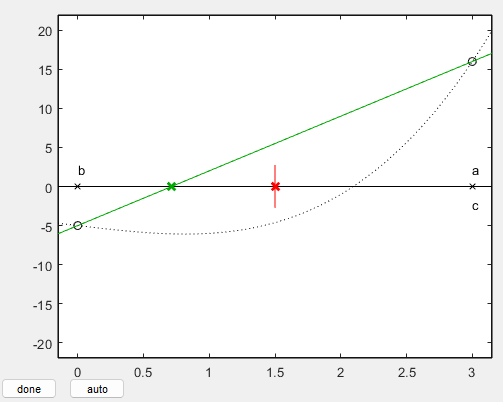
\includegraphics[width=0.8\textwidth]{Include/Images/Thesis/Development/Visualizers/NON LINEAR VISUALIZER/Mathworks.NonLinear.Ex1.png}
    \caption{Mathwork's \cite{doi:10.1137/1.9780898717952} NonLinear Visualizer Example}
    \label{fig:Mathwork's NonLinear Visualizer Example}
\end{figure}

\begin{figure}[H]
    \centering
    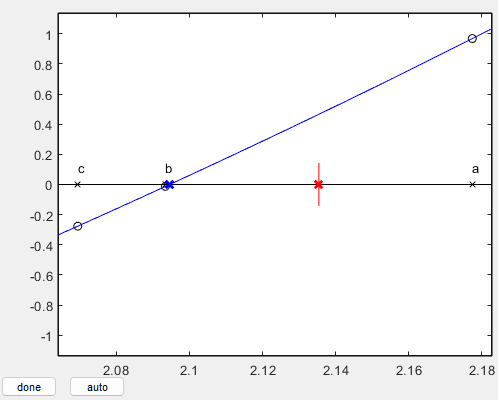
\includegraphics[width=0.8\textwidth]{Include/Images/Thesis/Development/Visualizers/NON LINEAR VISUALIZER/Mathworks.NonLinear.Ex1.1.png}
    \caption{Mathwork's \cite{doi:10.1137/1.9780898717952} NonLinear Visualizer Example - Ending}
    \label{fig:Mathwork's NonLinear Visualizer Example - Ending}
\end{figure}

We have adopted the same approach as Mathworks by adopting the algorithm established by Brent, Dekker, and his colleagues in our BNumMet implementation. We also took Mathwork's considerations, but extended and corrected the critiques we made previously. To solve the distinction between the points, we added a legend to indicate which point is which, and we moved the "interactivity" of the points to an external button so that the user knows what he is clicking on in every iteration \imgref{fig:BNumMet's NonLinear Visualizer Example}. We've also included a checkbox to the right of those buttons to enable the user choose whether to display the graph linked with the secant, I.Q.I, or bisection \imgref{fig:BNumMet's NonLinear Visualizer Example - Graphs for points }. It is also worth noting that we present what the original algorithm would be using, as well as information on the current solution the user has discovered and the amount of iterations the user has taken. It is worth noting that during each step the graph will resize accordingly for the user to properly visualize it. 


\begin{figure}[H]
    \centering
    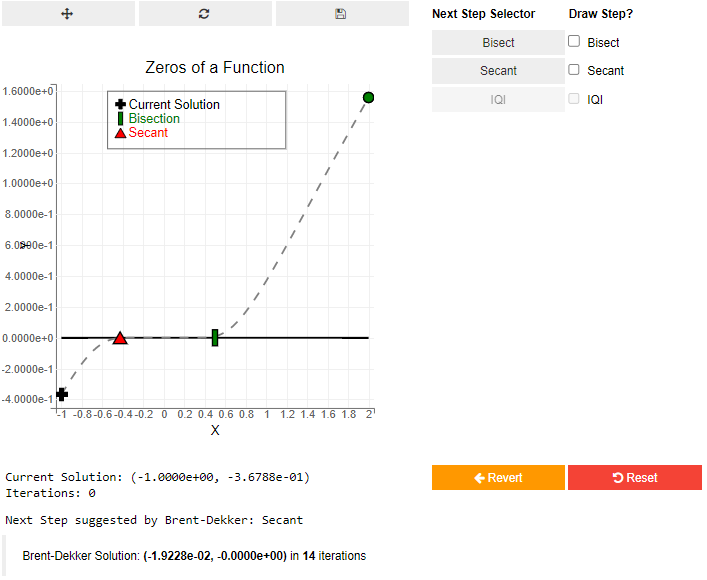
\includegraphics[width=\textwidth]{Include/Images/Thesis/Development/Visualizers/NON LINEAR VISUALIZER/BNumMet.NonLinear.Ex1.png}
    \caption{BNumMet's NonLinear Visualizer Example 1 }
    \label{fig:BNumMet's NonLinear Visualizer Example}
\end{figure}
\begin{figure}[H]
    \centering
    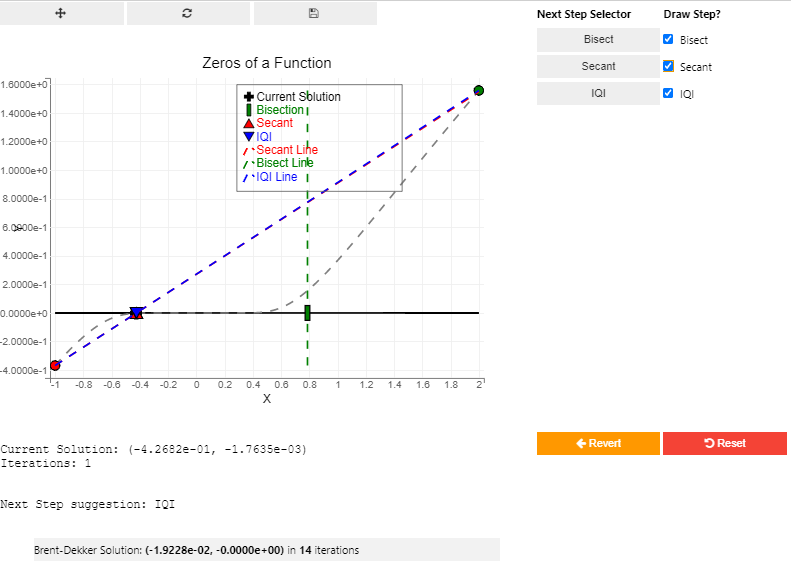
\includegraphics[width=\textwidth]{Include/Images/Thesis/Development/Visualizers/NON LINEAR VISUALIZER/BNumMet.NonLinear.Ex1.1.png}
    \caption{BNumMet's NonLinear Visualizer Example 1 - Graphs for points }
    \label{fig:BNumMet's NonLinear Visualizer Example - Graphs for points }
\end{figure}
\begin{figure}[H]
    \centering
    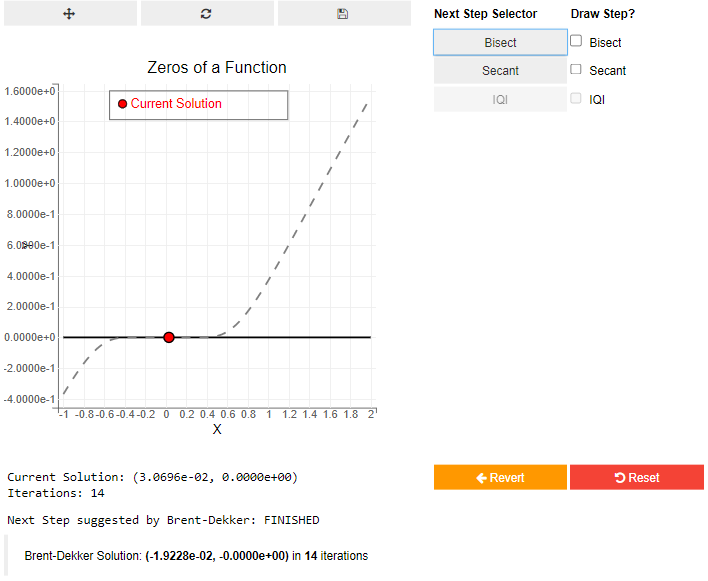
\includegraphics[width=\textwidth]{Include/Images/Thesis/Development/Visualizers/NON LINEAR VISUALIZER/BNumMet.NonLinear.Ex1.2.png}
    \caption{BNumMet's NonLinear Visualizer Example - Ending }
    \label{fig:BNumMet's NonLinear Visualizer Example - Ending }
\end{figure}
\subsubsection{Examples}
	\paragraph{Example 1: No arguments}
\begin{lstlisting}[language=Python]
from BNumMet.Visualizers.NonLinearVisualizer import NonLinearVisualizer
zerosVisualizer = NonLinearVisualizer()
zerosVisualizer.run()
\end{lstlisting}
\begin{enumerate}
    \item Initial State\\
    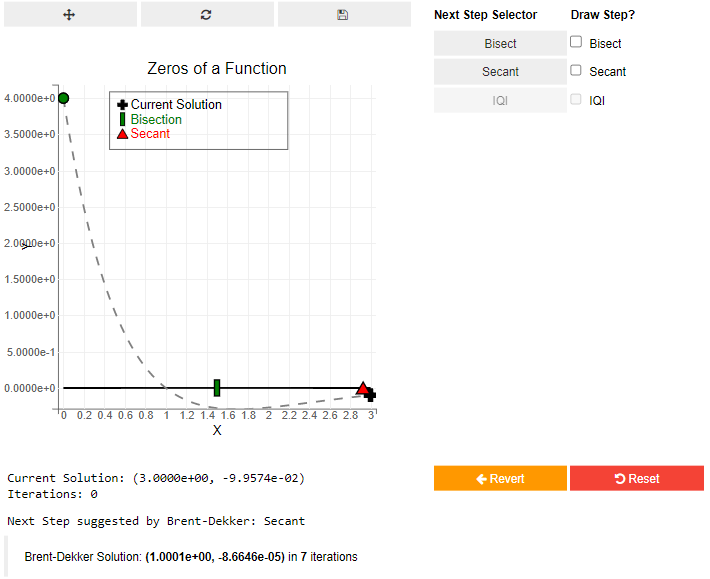
\includegraphics[width=0.8\textwidth]{Include/Images/Thesis/Documentation/Visualizers/NonLinear/Example 1/Example 1 - 00 - Initial State.png}
    \item Click on bisection checkbox\\
    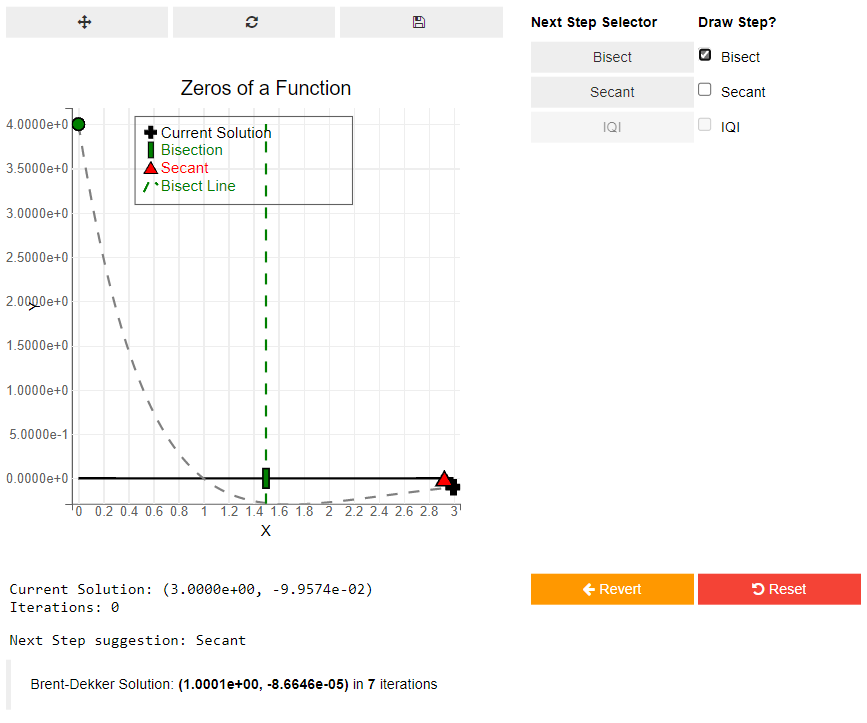
\includegraphics[width=0.8\textwidth]{Include/Images/Thesis/Documentation/Visualizers/NonLinear/Example 1/Example 1 - 01 - Bisection Checkbox.png}
    \item Click Secant Button\\
    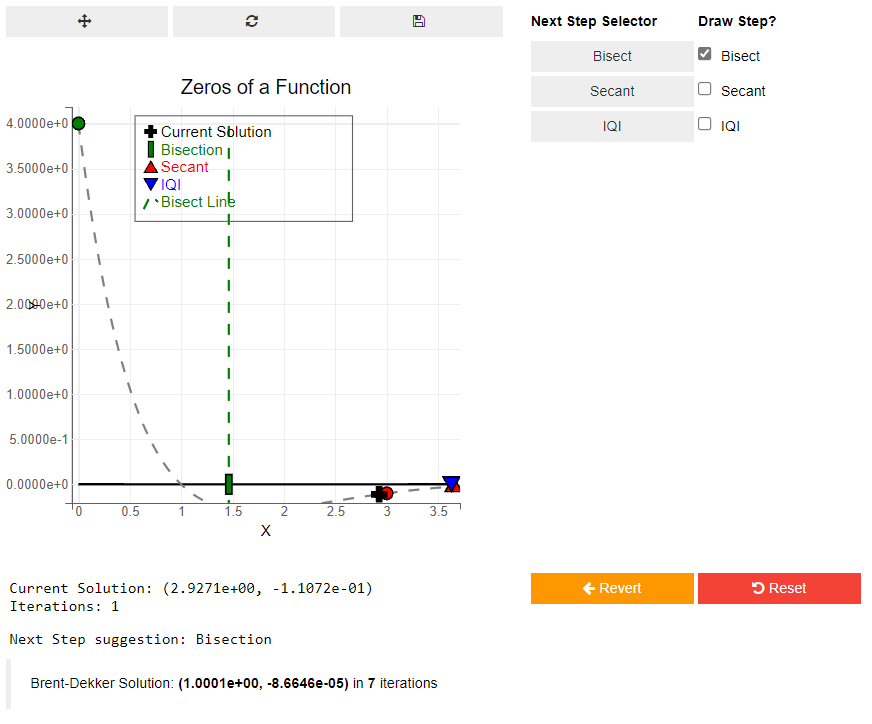
\includegraphics[width=0.8\textwidth]{Include/Images/Thesis/Documentation/Visualizers/NonLinear/Example 1/Example 1 - 02 - Click Secant.png}
    \item Some iterations after with secant checkbox clicked\\
    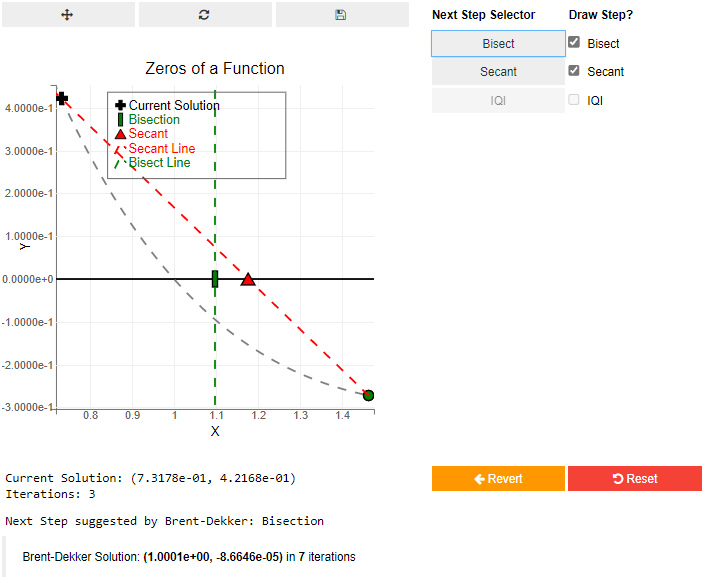
\includegraphics[width=0.8\textwidth]{Include/Images/Thesis/Documentation/Visualizers/NonLinear/Example 1/Example 1 - 03 - SOme iterations with secant checkbox.png}
    \item IQI Checkbox Only\\
    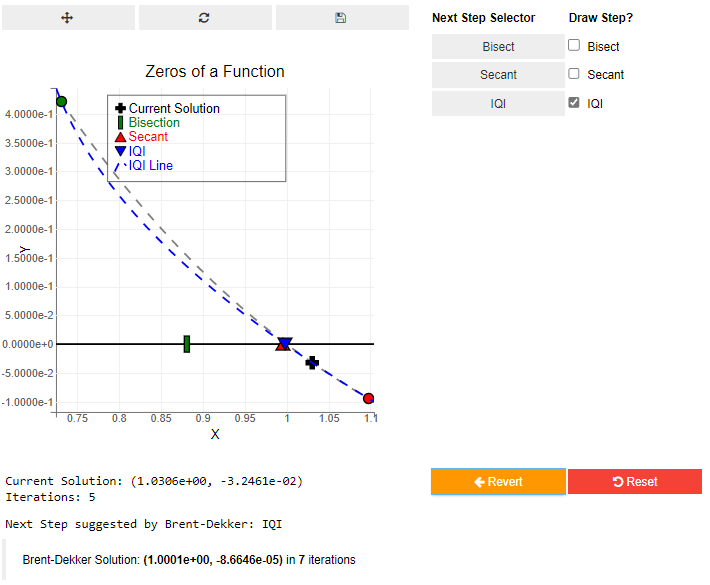
\includegraphics[width=0.8\textwidth]{Include/Images/Thesis/Documentation/Visualizers/NonLinear/Example 1/Example 1 - 04 - IQI checkbox only.png}

    \item Finished after some iterations\\
    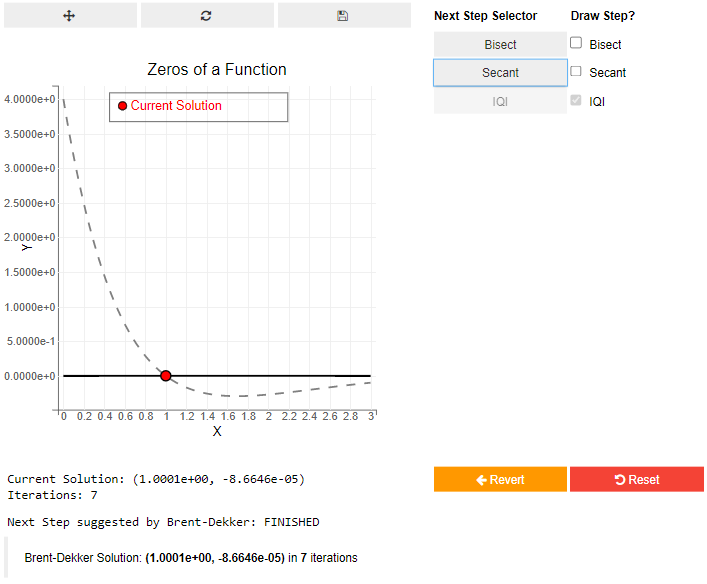
\includegraphics[width=0.8\textwidth]{Include/Images/Thesis/Documentation/Visualizers/NonLinear/Example 1/Example 1 - 04 - Finished.png}
   
\end{enumerate}



\paragraph{Example 2: With Arguments}
\begin{lstlisting}[language=Python]
from BNumMet.Visualizers.NonLinearVisualizer import NonLinearVisualizer
f2 = lambda x: 0 if abs(x) < 3.8 * 10 ** (-4) else float(x * np.exp(-1 / x**2))
interval = (-1, 2)
zerosVisualizer = NonLinearVisualizer(f2,interval)
zerosVisualizer.run()
\end{lstlisting}

\begin{enumerate}
    \item Initial State\\
    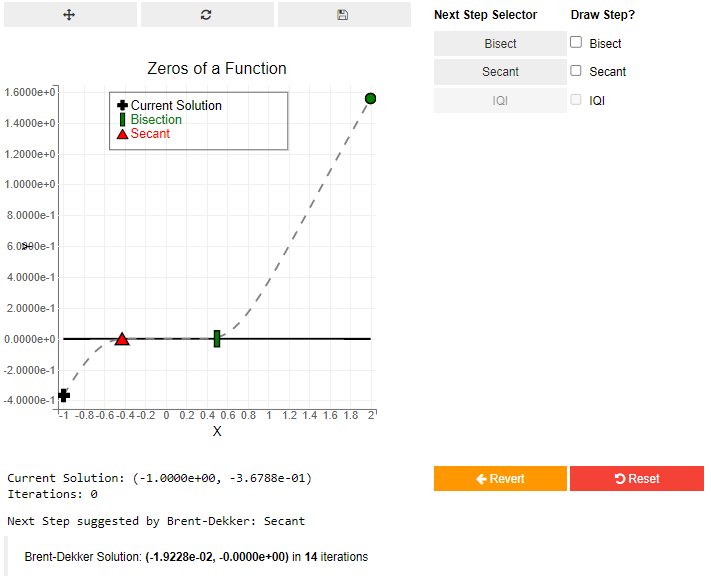
\includegraphics[width=0.8\textwidth]{Include/Images/Thesis/Documentation/Visualizers/NonLinear/Example 2/Example 2 - 00 - Initial State.png}
    \item All Checkboxes checked\\
    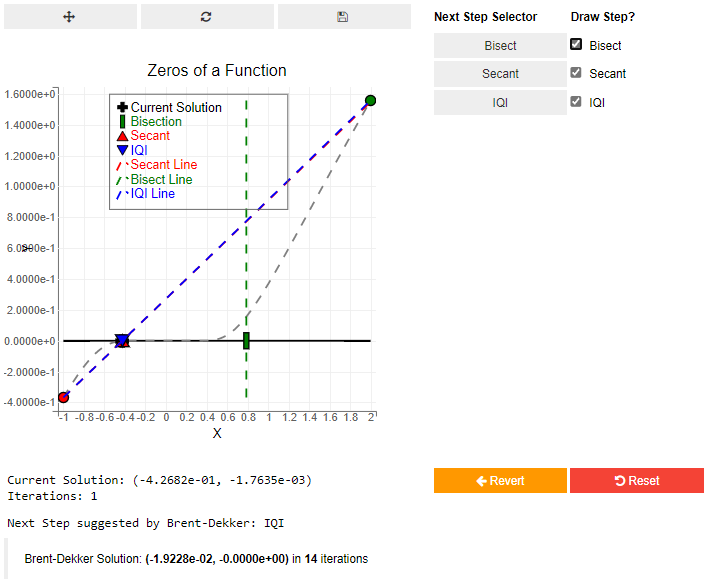
\includegraphics[width=0.8\textwidth]{Include/Images/Thesis/Documentation/Visualizers/NonLinear/Example 2/Example 2 - 01 - All Check Boxes.png}
    \item Click secant and click select all checkboxes again\\
    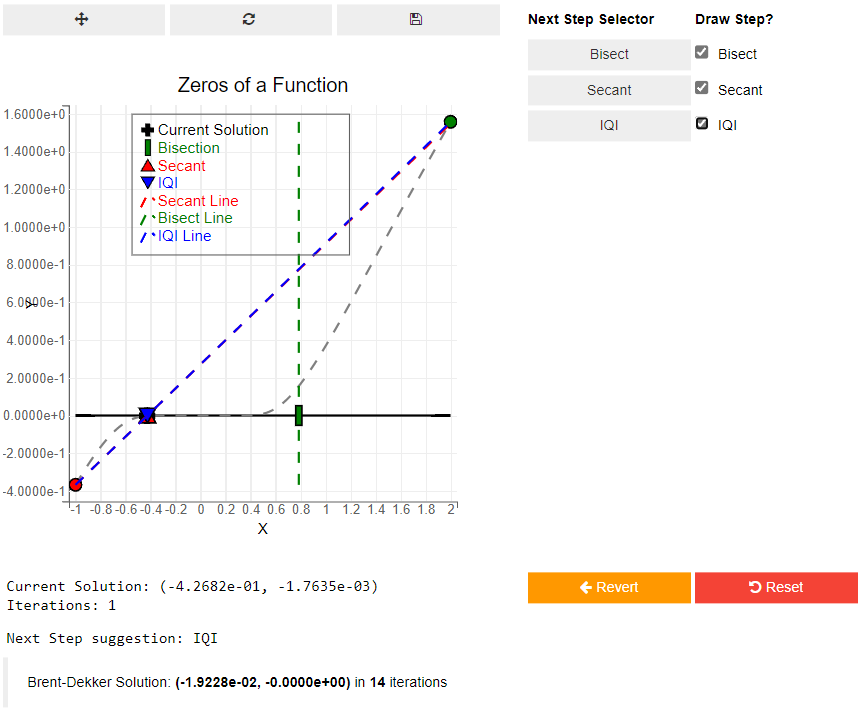
\includegraphics[width=0.8\textwidth]{Include/Images/Thesis/Documentation/Visualizers/NonLinear/Example 2/Example 2 - 02 - Click secant and All Check Boxes.png}
    \item Revert Button\\
    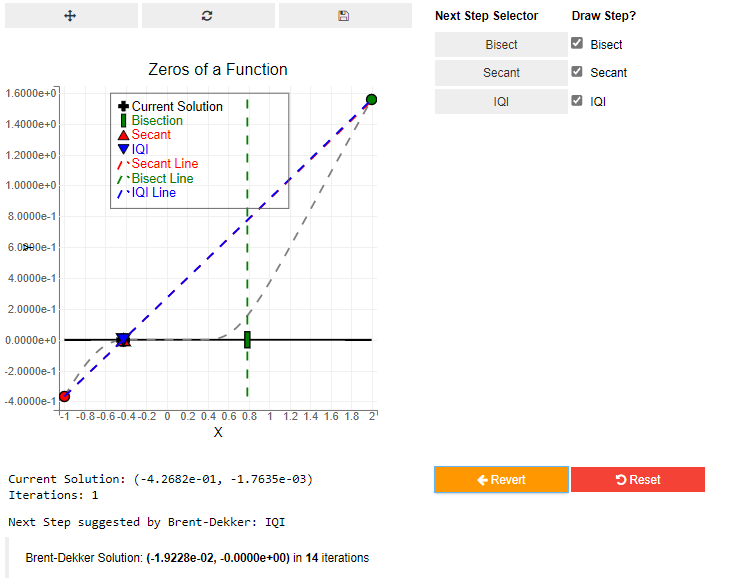
\includegraphics[width=0.8\textwidth]{Include/Images/Thesis/Documentation/Visualizers/NonLinear/Example 2/Example 2 - 03 - Revert Button.png}
    \item Some iterations\\
    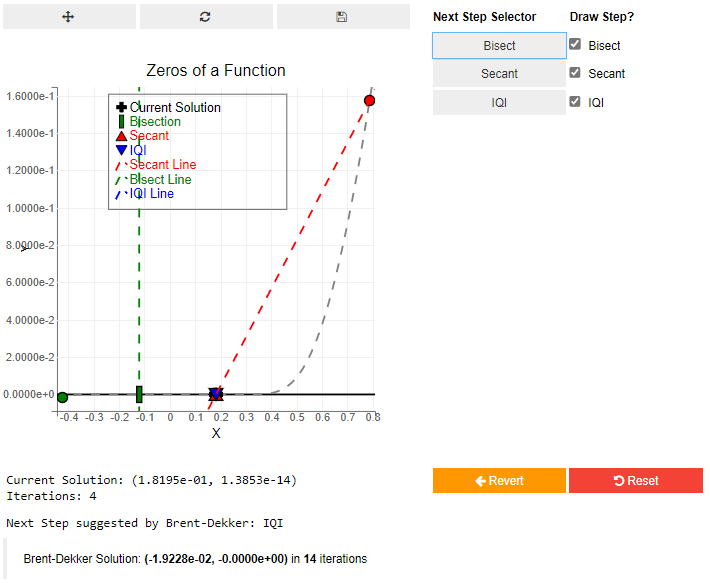
\includegraphics[width=0.8\textwidth]{Include/Images/Thesis/Documentation/Visualizers/NonLinear/Example 2/Example 2 - 04 - Some Iterations.png}
    \item Reset Button clicked\\
    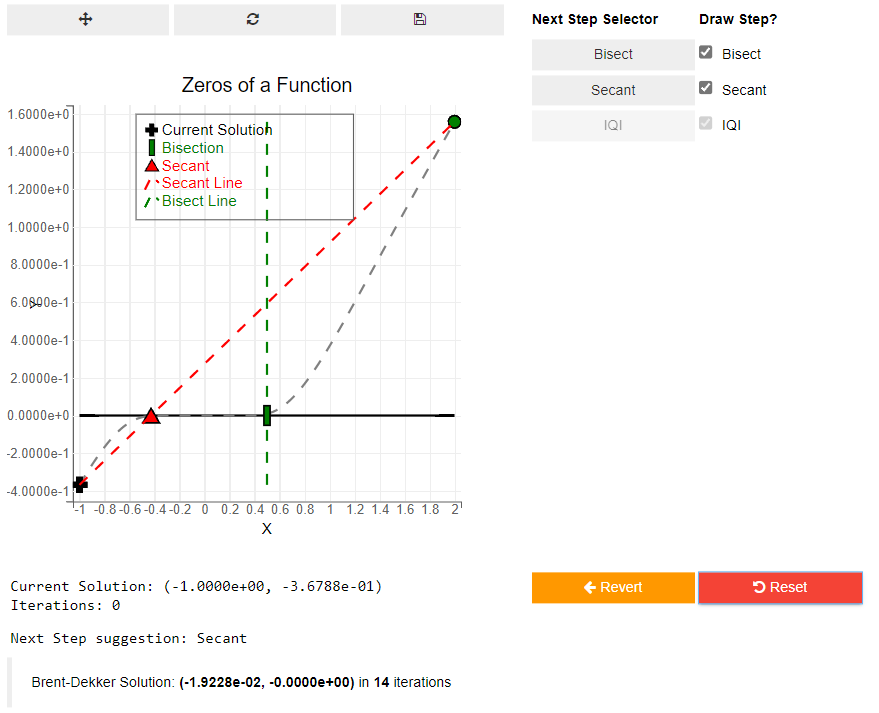
\includegraphics[width=0.8\textwidth]{Include/Images/Thesis/Documentation/Visualizers/NonLinear/Example 2/Example 2 - 04 - Reset Button.png}
    \item Finished after some iterations\\
    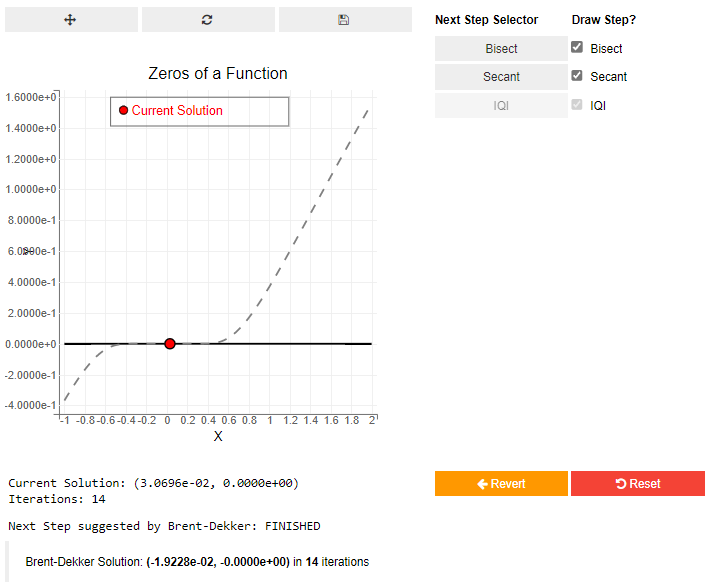
\includegraphics[width=0.8\textwidth]{Include/Images/Thesis/Documentation/Visualizers/NonLinear/Example 2/Example 2 - 05 - Finished.png}
\end{enumerate}


\subsection{Least Squares Problem Visualizer}
Although no mention of Least Squares was made during the discussion of the multiple numerical methods that BNumMet has, this problem is one of the pinnacles of data fitting and a complex problem with a simple approach to solve. As a result, we felt it was necessary to create a visualizer to give students with a complete and interactive tool to examine what least squares perform.

The main idea of the visualizer is to give the student a set of points (or allow them to enter their own data) and show them how to solve the least squares problem using various types of functions. All of the calculations will be done in the background while the final plot will be shown to demonstrate that in these types of problems, the goal is not to interpolate but to find a function that minimizes the error.

As with the previous visualizer, we will begin by discussing Mathwork's implementation; in this case, C. Moller's work is outstanding; he provides data from the US Census and presents the user with a selector of two functions for applying least squares and another two that interpolate the points. It also offers an estimate of the inaccuracy for each approach. It should be noted that it does not include the resultant equation that yields the least squares solution, which may be valuable for any learner checking their own hand-made computations.

\begin{figure}[H]
    \centering
    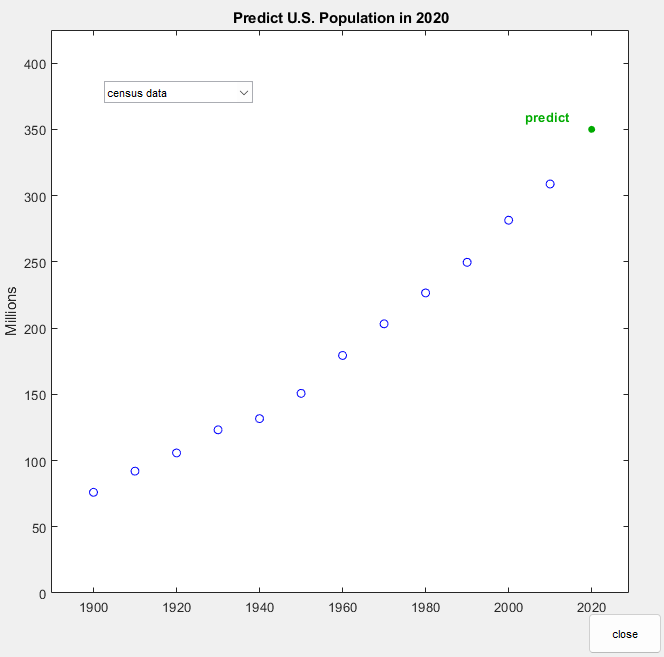
\includegraphics[width=0.6\textwidth]{Include/Images/Thesis/Development/Visualizers/LSP/Mathworks.LSP.Ex1.png}
    \caption{Mathwork's \cite{doi:10.1137/1.9780898717952} LSP Visualizer Example 1 - Data}
    \label{fig:Mathwork's NonLinear Visualizer Example - Data}
\end{figure}
\begin{figure}[H]
    \centering
    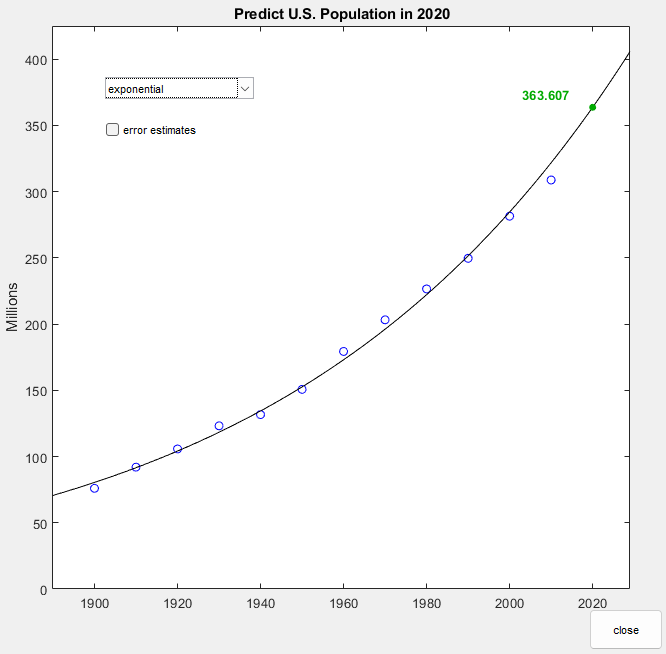
\includegraphics[width=0.6\textwidth]{Include/Images/Thesis/Development/Visualizers/LSP/Mathworks.LSP.Ex1.2.png}
    \caption{Mathwork's \cite{doi:10.1137/1.9780898717952} LSP Visualizer Example - Exponential}
    \label{fig:Mathwork's Least Squares Visualizer Example - Exponential}
\end{figure}
\begin{figure}[H]
    \centering
    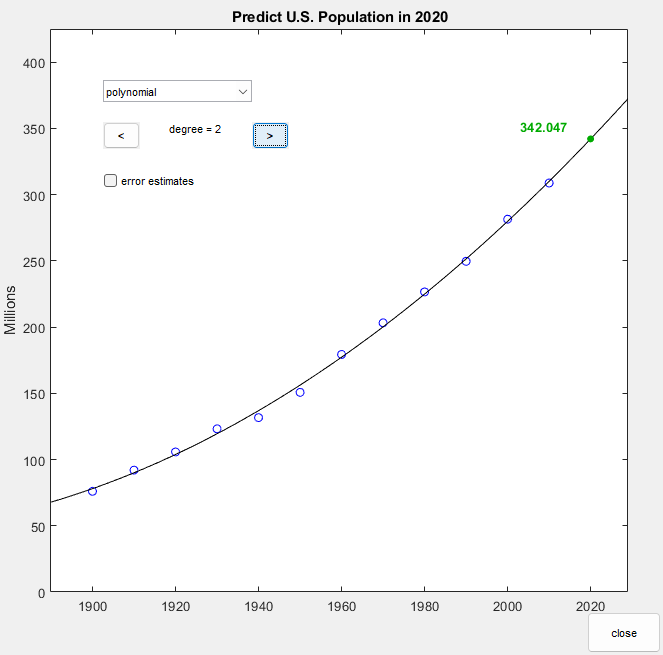
\includegraphics[width=0.6\textwidth]{Include/Images/Thesis/Development/Visualizers/LSP/Mathworks.LSP.Ex1.3.png}
    \caption{Mathwork's \cite{doi:10.1137/1.9780898717952} LSP Visualizer Example - Polynomial}
    \label{fig:Mathwork's Least Squares Visualizer Example- Polynomial}
\end{figure}

We generalized this approach in BNumMet's implementation by implementing just the techniques that relate to the real least squares issue, rather than the interpolating methods supplied in the interpolation package. We also noticed that, while Mathwork's approach demonstrated an interesting application about predicting the future of the population of the United States, it lacked the ability for the user to input their own data set, which we fixed in BNumMet's implementation and it may be regarded as a more interesting approach for students while learning.  In addition, we added a little note indicating the output function as well as the inaccuracy that the solution presents. We would also like to mention that we added the Sines and Cosines Basis for this problem since we thought it would provide insight into the fact that the least squares problem is not limited to a small set of functions but includes many more.

\begin{figure}[H]
    \centering
    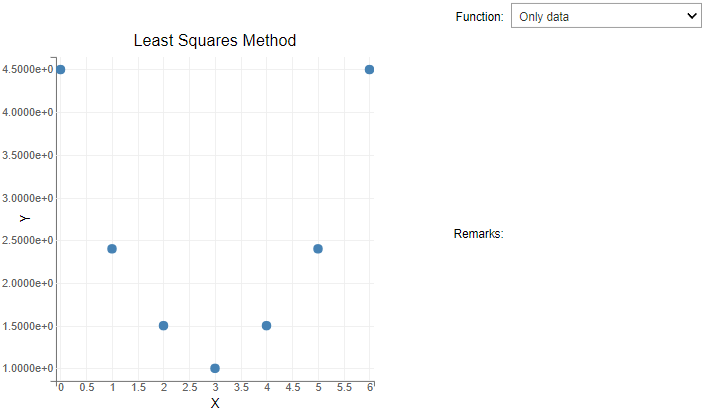
\includegraphics[width=0.8\textwidth]{Include/Images/Thesis/Development/Visualizers/LSP/BNumMet.LSP.Ex1.png}
    \caption{BNumMet's LSP Visualizer Example }
    \label{fig:BNumMet's Least Squares Visualizer Example}
\end{figure}
\begin{figure}[H]
    \centering
    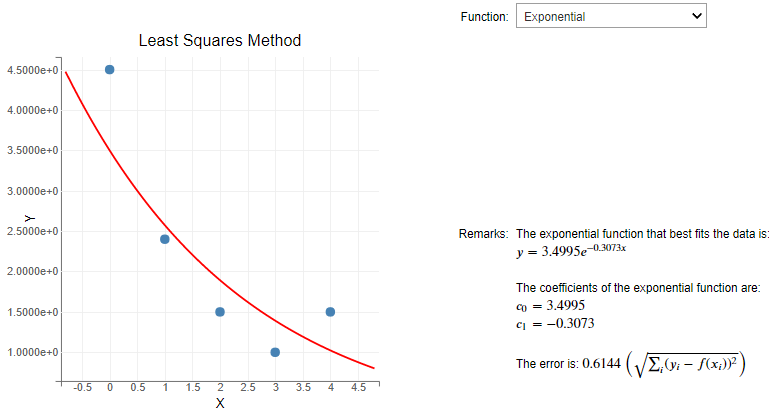
\includegraphics[width=0.8\textwidth]{Include/Images/Thesis/Development/Visualizers/LSP/BNumMet.LSP.Ex1.1.png}
    \caption{BNumMet's LSP Visualizer Example - Exponential}
    \label{fig:BNumMet's Least Squares Visualizer Example- Exponential}
\end{figure}
\begin{figure}[H]
    \centering
    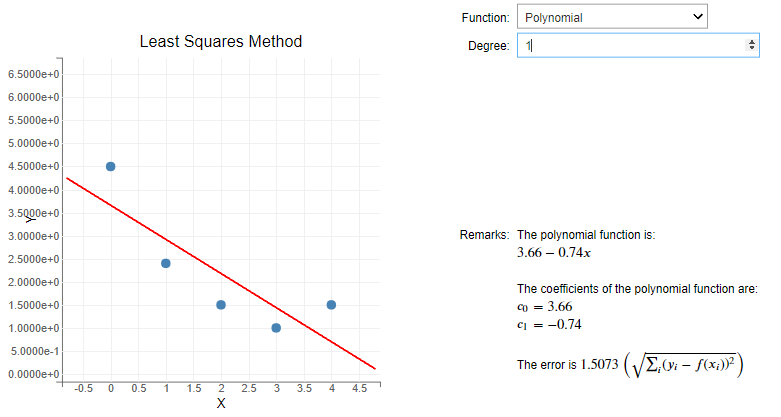
\includegraphics[width=0.8\textwidth]{Include/Images/Thesis/Development/Visualizers/LSP/BNumMet.LSP.Ex1.2.png}
    \caption{BNumMet's LSP Visualizer Example - Polynomial}
    \label{fig:BNumMet's Least Squares Visualizer Example- Polynomial}
\end{figure}
\begin{figure}[H]
    \centering
    \includegraphics[width=0.8\textwidth]{Include/Images/Thesis/Development/Visualizers/LSP/BNumMet.LSP.Ex1.3.png}
    \caption{BNumMet's LSP Visualizer Example - Sines and Cosines}
    \label{fig:BNumMet's Least Squares Visualizer Example- Sines and Cosines}
\end{figure}
As we can see we have removed the error estimates that Mathwork's implementation presents, we believed it may be confusing and without a proper definition of how it is calculated.
\subsubsection{Examples}
	\paragraph{Example 1: Polynomial Fit of Varying degree}{
\begin{lstlisting}[language=Python]
from BNumMet.Visualizers.LeastSquaresVisualizer import LSPVisualizer
xData = np.array([0, 1, 2, 3, 4, 5])
yData = np.array([4.5, 2.4, 1.5, 1, 1.5, 2.4])
lspVisualizer = LSPVisualizer(xData, yData)
lspVisualizer.run()
\end{lstlisting}

\begin{enumerate}
    \item Initial State\\
    \includegraphics[scale=0.6]{Include/Images/Thesis/Documentation/Visualizers/LeastSquares/Example 1/Example 1 - 00 - Initial State.png}
    \item Selector\\
    \includegraphics[scale=0.6]{Include/Images/Thesis/Documentation/Visualizers/LeastSquares/Example 1/Example 1 - 00 - Selector.png}
    \item Select Polynomial\\
    \includegraphics[scale=0.6]{Include/Images/Thesis/Documentation/Visualizers/LeastSquares/Example 1/Example 1 - 00 - Polinomial .png}
    \item Increment degree by 1 (degree 2)\\
    \includegraphics[scale=0.6]{Include/Images/Thesis/Documentation/Visualizers/LeastSquares/Example 1/Example 1 - 01 - Polinomial Degree 2.png}
    \item Degree 5 (Maximum, cannnot go higher)\\
    \includegraphics[scale=0.6]{Include/Images/Thesis/Documentation/Visualizers/LeastSquares/Example 1/Example 1 - 02 - Polinomial Degree 5.png}

\end{enumerate}
}

\paragraph{Example 2: No Input Data and Exponential Fit}
\begin{lstlisting}[language=Python]
from BNumMet.Visualizers.LeastSquaresVisualizer import LSPVisualizer
lspVisualizer = LSPVisualizer()
lspVisualizer.run()
\end{lstlisting}
\begin{enumerate}
    \item Initial state\\
    \includegraphics[scale=0.6]{Include/Images/Thesis/Documentation/Visualizers/LeastSquares/Example 2/Example 2 - 00 - Initial State.png}
    \item Exponential Selection\\
    \includegraphics[scale=0.6]{Include/Images/Thesis/Documentation/Visualizers/LeastSquares/Example 2/Example 2 - 00 - Exponential.png}
\end{enumerate}

\paragraph{Example 3: Sines and Cosines Fit of Varying degree}{
\begin{lstlisting}[language=Python]
from BNumMet.Visualizers.LeastSquaresVisualizer import LSPVisualizer
xData = np.array([0, 1, 2, 3, 4, 5])
yData = np.array([4.5, 2.4, 1.5, 1, 1.5, 2.4])
lspVisualizer = LSPVisualizer(xData, yData)
lspVisualizer.run()
\end{lstlisting}

\begin{enumerate}
    \item Initial State\\
    \includegraphics[scale=0.6]{Include/Images/Thesis/Documentation/Visualizers/LeastSquares/Example 1/Example 1 - 00 - Initial State.png}
    \item Selector\\
    \includegraphics[scale=0.6]{Include/Images/Thesis/Documentation/Visualizers/LeastSquares/Example 1/Example 1 - 00 - Selector.png}
    \item Select Sines \& Cosines\\
    \includegraphics[scale=0.6]{Include/Images/Thesis/Documentation/Visualizers/LeastSquares/Example 3/Example 3 - 00 - Trigonometry.png}
    \item Set degree to the maximum\\
    \includegraphics[scale=0.6]{Include/Images/Thesis/Documentation/Visualizers/LeastSquares/Example 3/Example 3 - 01 - Trigonometry Degree 2.png}
\end{enumerate}
}


\subsection{Random Visualizer}
A part of applied mathematics outreach is the common application that goes as follows, throw at random n-number of darts inside a square with an inner circle with diameter the size of the square, when computing the number of darts that are inside the circle and the ones outside, one can with more or less accuracy find the value of $\pi$. For this reason we will implement this simple game as part of the random visualization package, to show students the power of Montecarlo's Simulation, that is, we will implement a target and using a random number generator we will simulate the throwing of darts to then observe how we obtain pi.

First, as with the other visualizers, we examine Mathwork's implementation; in this case, C. Moller chose a 3D version of the game; the method allows for the input of different types of generators; however, we must note that this implementation does not allow for varying the number of points, but it does allow for the simulation to be repeated.

\begin{figure}[H]
    \centering
    \includegraphics[width=0.8\textwidth]{Include/Images/Thesis/Development/Visualizers/RANDOMNESS/Mathworks.Random.Ex1.png}
    \caption{Mathwork's \cite{doi:10.1137/1.9780898717952} Random Visualizer Example}
    \label{fig:Mathwork's Random Visualizer Example}
\end{figure}

A similar implementation was done in BNumMet, but in this instance we used the 2D method since we believe the students would find it easier to grasp, observe, and even write it themselves. We allowed the user to select the number of points they wanted to toss as part of the implementation. We have provided a graph that depicts how the simulation approaches $\pi$. To address the major issue with Mathwork's, we created a button that allows the user to run the simulation with the specified number of points anytime they want. And, as C. Moller suggested, we included the value of pi obtained when the program iterated. One disadvantage of BNumMet's implementation over C. Moller's is that we must restrict the number of points to 10000 since for such numbers the animation takes very long. That is why we chose to implement the Montecarlo Simulation with batches, that is, with an n-sized batch that saves the data until they reach the appropriate length and then updates the animation.
\begin{figure}[H]
    \centering
    \includegraphics[width=\textwidth]{Include/Images/Thesis/Development/Visualizers/RANDOMNESS/BNumMet.Random.Ex1.png}
    \caption{BNumMet's Random Visualizer Example}
    \label{fig:BNumMet's Random Visualizer Example}
\end{figure}
\subsubsection{Examples}
	\paragraph{Example 1: No input arguments}
\begin{lstlisting}[language=Python]
from BNumMet.Visualizers.RandomVisualizer import RandomVisualizer
randomVisualizer = RandomVisualizer()
randomVisualizer.run()
\end{lstlisting}

\begin{enumerate}
    \item Initial State\\
    \includegraphics[scale=0.7]{Include/Images/Thesis/Documentation/Visualizers/Randomness/Example 1/Example 1 - 00 - Initial State.png}
    \item Clicked played with 100 default points\\
    \includegraphics[scale=0.7]{Include/Images/Thesis/Documentation/Visualizers/Randomness/Example 1/Example 1 - 01 - Clicked PLayed.png}
    \item Change number of points to 500 and clicked play\\
    \includegraphics[scale=0.7]{Include/Images/Thesis/Documentation/Visualizers/Randomness/Example 1/Example 1 - 02 - Changed N of points and played.png}
    \item Final of animation playing\\
    \includegraphics[scale=0.7]{Include/Images/Thesis/Documentation/Visualizers/Randomness/Example 1/Example 1 - 03 - Finished.png}
\end{enumerate}


\paragraph{Example 2: Input arguments and Ill-Generator}
\begin{lstlisting}[language=Python]
from BNumMet.Visualizers.RandomVisualizer import RandomVisualizer
from BNumMet.Random import marsaglia_rand, clear_marsaglia_vars

clear_marsaglia_vars()
randomFunc = lambda: marsaglia_rand(
    base=10, lag_r=2, lag_s=1, carry=0, seed_tuple=(0, 1)
)
randomVisualizer = RandomVisualizer(randomFunc)
randomVisualizer.run()
\end{lstlisting}

\begin{enumerate}
    \item Initial State\\
    \includegraphics[scale=0.7]{Include/Images/Thesis/Documentation/Visualizers/Randomness/Example 2/Example 2 - 00 - Initial State.png}
    \item Clicked played with 100 default points\\
    \includegraphics[scale=0.7]{Include/Images/Thesis/Documentation/Visualizers/Randomness/Example 2/Example 2 - 01 - Clicked PLayed.png}
    \item Change number of points to 1000 and clicked play\\
    \includegraphics[scale=0.7]{Include/Images/Thesis/Documentation/Visualizers/Randomness/Example 2/Example 2 - 02 - 1000 points played.png}

\end{enumerate}
